\documentclass[Royal,times,sageh]{sagej}

\usepackage{moreverb,url,natbib, multirow, tabularx}
\usepackage[colorlinks,bookmarksopen,bookmarksnumbered,citecolor=red,urlcolor=red]{hyperref}



% tightlist command for lists without linebreak
\providecommand{\tightlist}{%
  \setlength{\itemsep}{0pt}\setlength{\parskip}{0pt}}



\usepackage[utf8]{inputenc}
\usepackage[T1]{fontenc}



\begin{document}


\setcitestyle{aysep={,}}

\title{The bot that makes history}

\runninghead{Falk \emph{et al}.}

\author{Michael Falk*\affilnum{1}, Heather Ford\affilnum{1}, Tamson
Pietsch\affilnum{2}, Nathaniel Tkacz\affilnum{3}}

\affiliation{\affilnum{1}{Digital and Social Media, University of
Technology Sydney, Sydney, Australia}\\\affilnum{2}{Australian Centre
for Public History, University of Technology Sydney, Sydney,
Australia}\\\affilnum{3}{Centre for Interdisciplinary Methodologies,
University of Warwick, Conventry, United Kingdom}}

\corrauth{Michael Falk, Digital and Social Media, University of
Technology Sydney}

\email{\href{mailto:michael.falk@uts.edu.au}{\nolinkurl{michael.falk@uts.edu.au}}}


\keywords{Wikipedia; bots; temporal regime; time; historicity; trace
ethnography}

\maketitle

\hypertarget{introduction-wikipedia-and-the-technicity-of-time}{%
\section{Introduction: Wikipedia and The Technicity of
Time}\label{introduction-wikipedia-and-the-technicity-of-time}}

Time is a supple medium. It winds itself into many shapes. It surges
through the heartwood. It lies upon the bark. It carves rock and unfolds
in song. It creates myriad structures, then entropically destroys them.
It races, dallies, recurs, reverses, accelerates, splits and stops.

Despite its suppleness, time has definite characteristics. It forms
rhythms. It weaves people and plants and animals into lives and seasons.
It founds eras.

What are the characteristics of time in the digital era? The question
has been a major preoccupation for humanists and social scientists in
the twenty-first century. Theorists in many disciplines have argued that
`presentism' is the dominant `temporal regime' of the twenty-first
century \citep{assmann_is_2020, hartog_regimes_2017}. We inhabit a
`broad present' \citep{gumbrecht_our_2014} or a `timeless time'
\citep{castells_rise_2010} in which big data and frictionless
communication have conspired with the cult of memory to abolish the
future and bring the past into the present. We live in a rubble-world of
accumulating fact. Other theorists have diagnosed the problem as
`temporal acceleration'. We experience time as running ever faster,
argues \citet[p.~77]{wajcman_pressed_2015}, because it has become
`deroutinized'. We are trapped in the present because we are present in
so many places at once: on the phone to daycare while picking up dinner
ingredients in the supermarket on our lunchbreak at work. Digital media
are the handmaidens of post-industrial capitalism. Without them, we
would be unable to maintain the modicum of order we currently enjoy.

A weakness of many theories of temporality is their focus on the
\emph{products} rather than the \emph{production} of temporal regimes.
To characterise a temporal regime, the theorist considers some cultural
products, such as literary texts
\citep{gumbrecht_our_2014, hartog_regimes_2017} or work-time statistics
\citep{castells_rise_2010} and tries to determine what kind of temporal
regime those products represent. Such accounts necessarily raise the
question: how is it possible to erect a temporal regime in the first
place? A compelling answer is given by \citet{orlikowski_its_2002}, who
argue that the temporal regime of an organisation is produced by the
`practices' of its members. Such practices can modify a temporal regime
`implicitly' or `explicitly' \citeyearpar[p.~687]{orlikowski_its_2002},
though in either case the key force of change is \emph{repetition}, or
`recurrent action' \citeyearpar[p.~696]{orlikowski_its_2002}. Temporal
regimes are rhythmical. They are produced by the recurrent actions of
people, who learn to act in concert as the members of an orchestra.

In this paper, we build on Orlikowski and Yates's theory of temporal
structuration to describe the temporal regime of Wikipedia. We show that
to explain Wikipedia's temporal regime, it is necessary to supplement
Orlikowski and Yates's theory of \emph{repetition} with a theory of
time's \emph{representation} and its \emph{technicity}. Only by
accounting for these three aspects of time can we adequately answer our
central questions: (1) what is Wikipedia time? and (2) what can it tell
us about digital time more broadly?

Our central case study is
\href{https://en.wikipedia.org/wiki/User:Yapperbot}{Yapperbot/uncurrenter},
a `bot' or computer program that polices the barrier between past and
present on English Wikipedia. We situate Yapperbot/uncurrenter in
Wikipedia's broader sociotechnical systems. We examine how it interacts
with human editors. We show how it fits into Wikipedia's complex array
of interfaces and data streams. We present Yapperbot/uncurrenter as a
prime example of the `technicity of time'. It is a technology that
attempts to make time concrete, to freeze it into an object.
Yapperbot/uncurrenter is like the master's clock in an
eighteenth-century factory. It ticks regularly (\emph{repetition}),
shows the time (\emph{representation}) and acts impersonally
(\emph{technicity}).

Yapperbot/uncurrenter performs a single, simple task. Each hour, it
scans English Wikipedia, finding every article that `transcludes'
\href{https://en.wikipedia.org/wiki/Template:Current}{Template:Current}.
If the article has not been edited in over five hours, it deletes the
template.

A `template' is a microprogram that peforms a common task. In the case
of Template:Current, the editor inserts the code
\texttt{\{\{current\}\}} into an article. This adds a warning banner to
the article (Figure \ref{fig:banner_collage}), and automatically adds
the article to
\href{https://en.wikipedia.org/wiki/Category:Current_events}{Category:Current\_events}.
When Yapperbot/uncurrenter deletes the template, the banner disappears,
as does the article's categorisation as a `current event'. This would
seem to consign the article to the past. But here lies the first twist
in the tale. When Yapperbot/uncurrenter deletes Template:Current, it
leaves an oddly contradictory message in the article's edit history:

\begin{quote}
Auto-removing \{\{current\}\} - no edits in 5hrs+. The event may still
be current, but
\href{https://en.wikipedia.org/wiki/Template:Current}{the
\{\{current\}\} template is designed only for articles which many
editors are editing, and is usually up for less than a day}.
\end{quote}

On English Wikipedia, an event can be `current' without being
\texttt{\{\{current\}\}}. This contradiction lies at the heart of
Wikipedia's temporal regime. When Wikipedia's English editors debated
the need for Yapperbot/uncurrenter, they ran straight into the
contradiction between two different understandings of time. To stabilise
Wikipedia's temporal regime, they had to resolve this contradiction. As
we show below, Wikipedia's English editors made the radical move to try
and abolish the present, a path that editors of other-language
Wikipedias have refused to take.

\begin{figure}
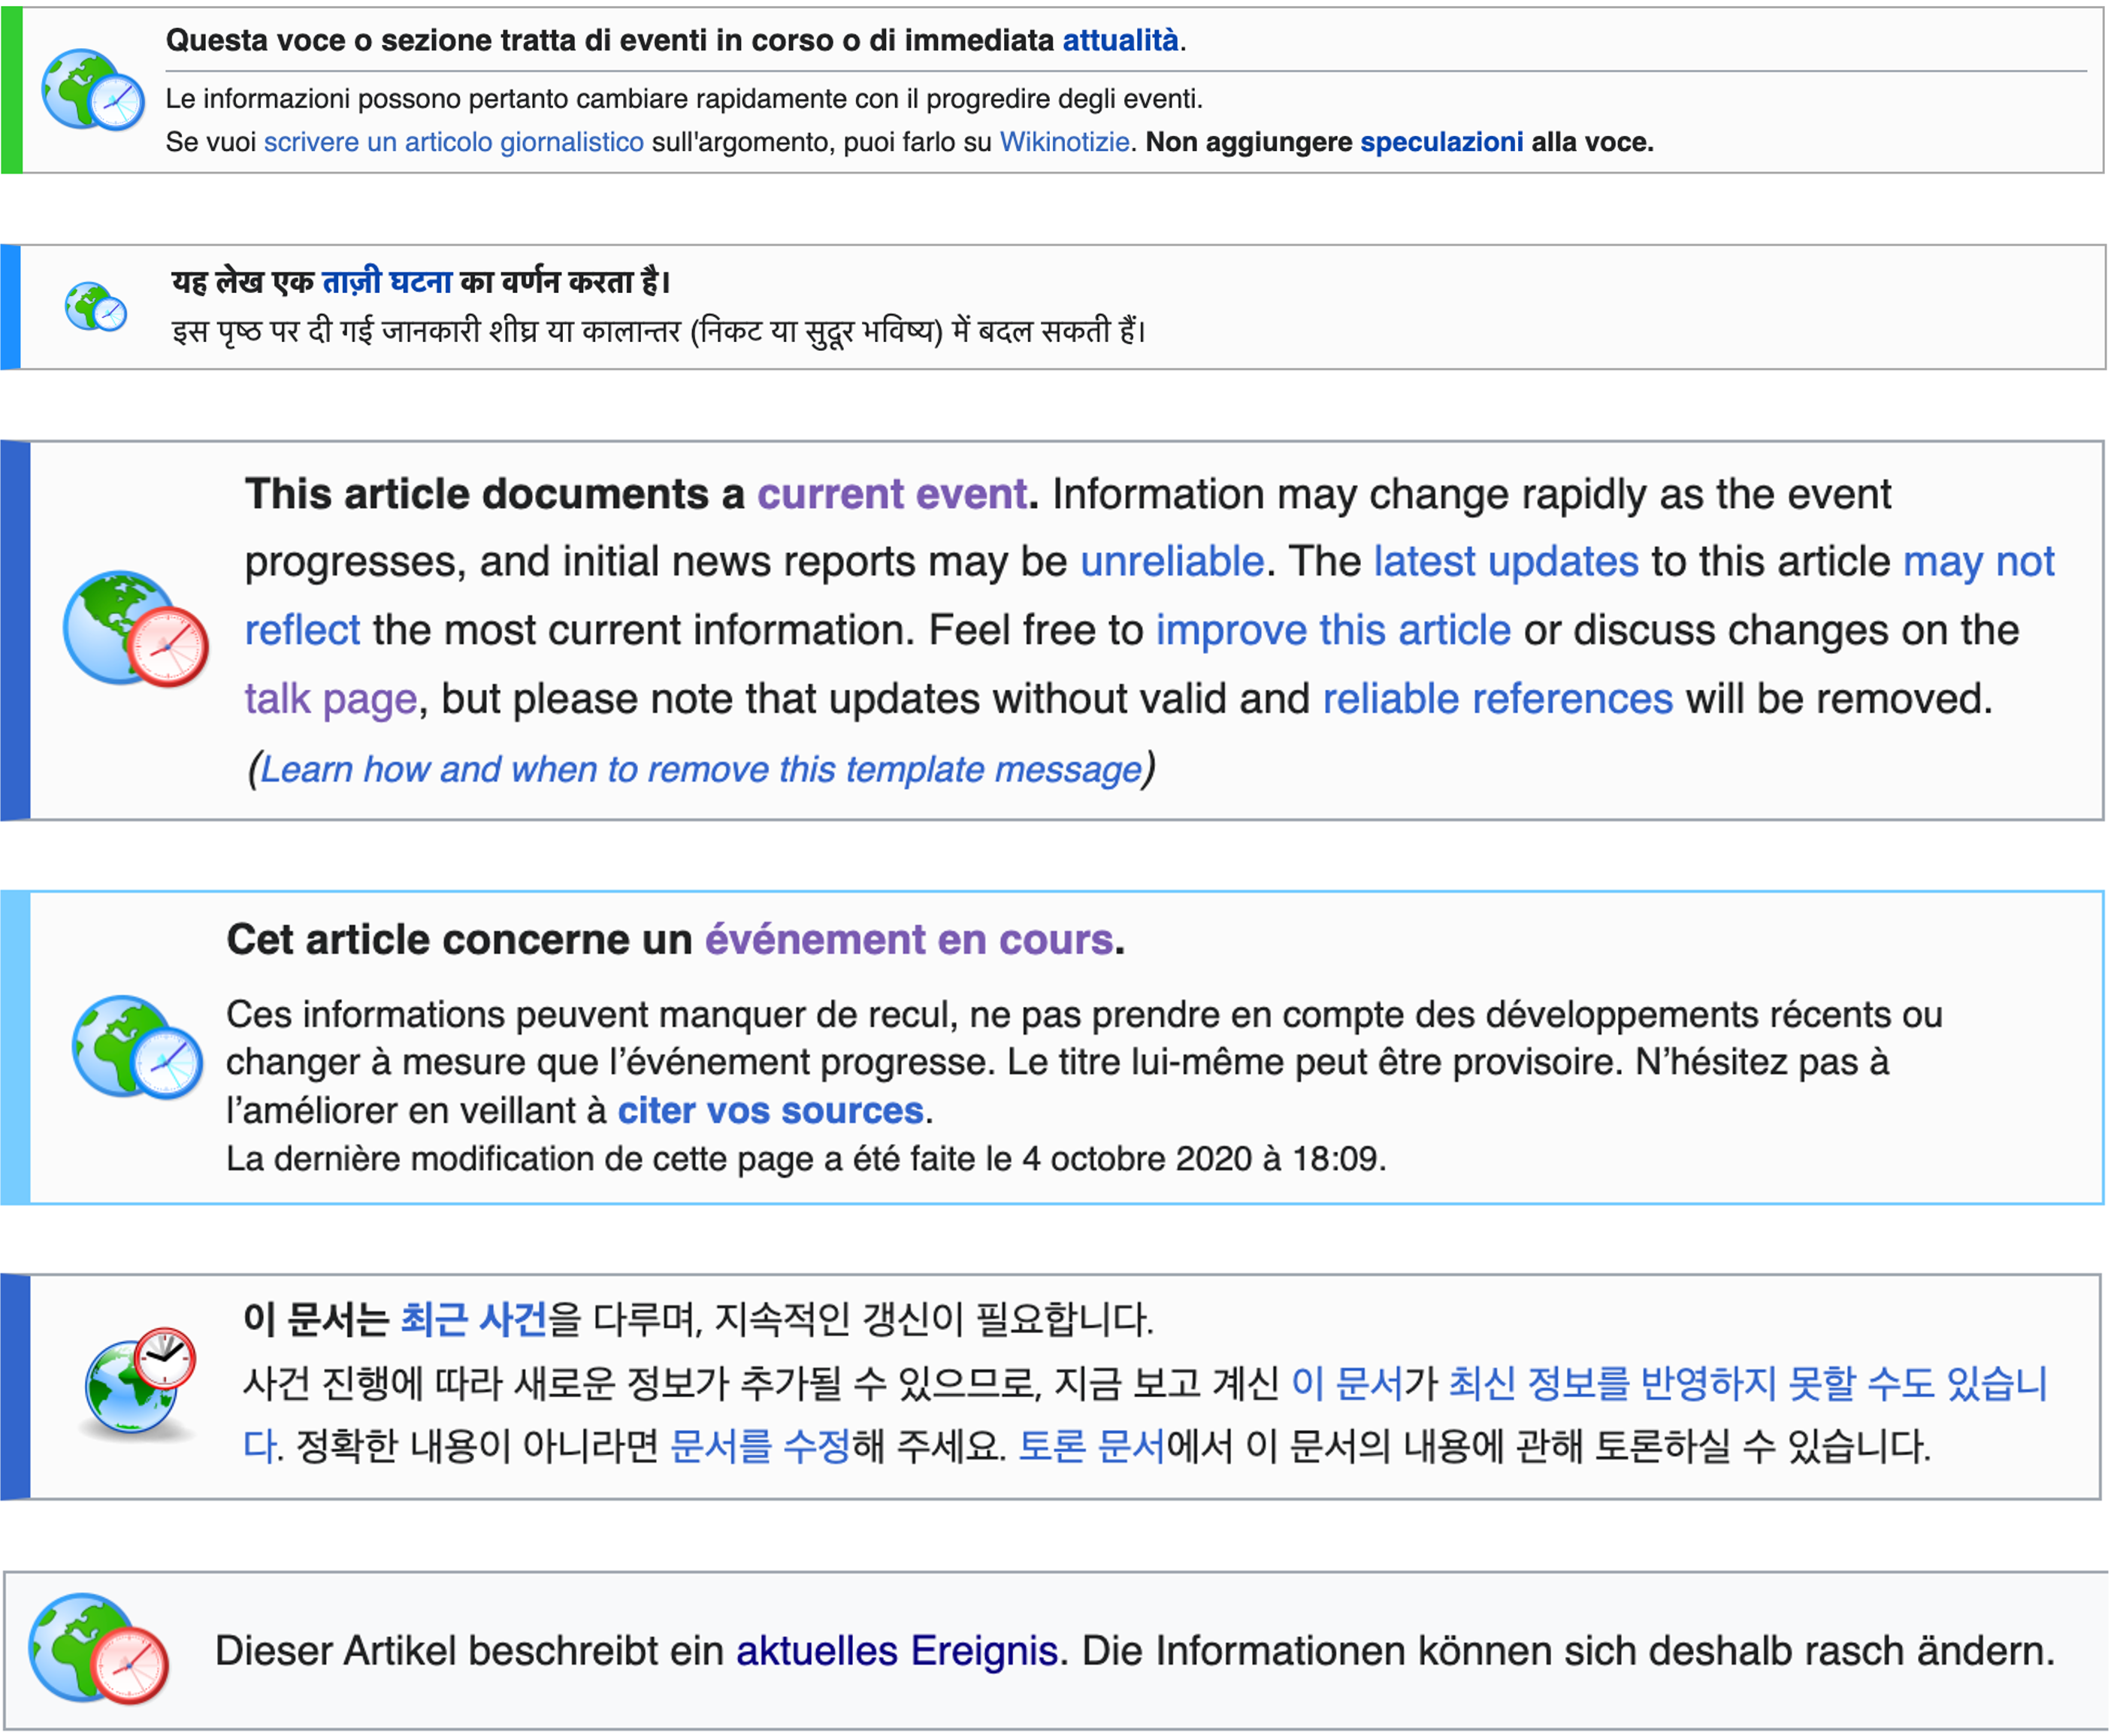
\includegraphics[width=1\linewidth]{images/banner_collage} \caption{Template:Current in Italian, Hindi, English, French, Korean and German (as of 14 March 2023)\label{fig:banner_collage}}\label{fig:unnamed-chunk-1}
\end{figure}

Wikipedia is one of the few places where where the construction of a
temporal regime can be (almost) directly observed. Unlike other
prominent social media platforms, Wikipedia is an `open' project, every
one of whose facets can be publicly altered and debated. The
encyclopaedia can only be changed in public. Nearly every step in the
construction of the temporal regime leaves an easily-recovered mark. It
may appear that an `open' platform such as Wikipedia could never
tolerate something as closed as a temporal \emph{regime}, but as
\citet{tkacz_wikipedia_2015} shows, Wikipedia's openness has not
prevented it from developing a restrictive `frame' of rules and concepts
that govern its activities. Quite the contrary. Wikipedia is not only
the most open of social networks---it is surely also the most highly
organised.

Wikipedia is also a place where `technicities of time' are especially
prominent. Large parts of the encyclopedia are managed by bots such as
Yapperbot/uncurrenter, which are powerful actors in Wikipedia's
sociotechnical system
\citetext{\citealp{niederer_wisdom_2010}; \citealp[pp.~137-140]{dijck_culture_2013}; \citealp{geiger_work_2010}; \citealp{geiger_when_2013}; \citealp[pp.~111-119]{tkacz_wikipedia_2015}; \citealp{geiger_operationalizing_2017}; \citealp{halfaker_bots_2012}; \citealp{livingstone_population_2016}}.
Bots are best understand as users of the platform, rather than as
extensions of their human developers. Indeed, Wikipedia bots have
ordinary user accounts like human Wikipedians, although they also have
special privileges and their actions are tracked separately by the
system. Bots incarnate or enact Wikipedia's culture, as Stuart Geiger
has revealed in a pathbreaking series of papers
\citetext{\citealp{geiger_social_2009}; \citealp{geiger_lives_2011}; \citealp{geiger_are_2013}; \citealp{geiger_beyond_2017}; \citealp[see
also][]{kennedy_textual_2010}}. To understand bots, he explains, it is
not sufficient to read the source code, although there may well be
important policies, procedures or ideals `encoded' in the source
\citeyearpar[p.~9]{geiger_beyond_2017}. Instead, it is essential to
observe how bots act in the wild, and to observe how human users and
other bots interact with \emph{them}
\citetext{\citeyear{geiger_lives_2011}; \citeyear{geiger_beyond_2017}}.
In this spirit, we pursue Yapperbot/uncurrenter through Wikipedia, to
see how it works and whom it fights to uphold Wikipedia's temporal
regime.

Our discussion falls into four main sections. In
\protect\hyperlink{how-to-make-time}{How to make time}, we present a
theory of `temporal mapping' to show how temporal regimes can be
produced through repetition, representation and technicity. In
\protect\hyperlink{wikipedia-time-1-the-primacy-of-the-past}{Wikipedia
time (1): the primacy of the past}, we consider existing research into
Wikipedia's temporal regime, and consider the various ways that time
enters into the encyclopaedia. In
\protect\hyperlink{the-birth-of-the-bot-that-makes-history}{The birth of
the bot that makes history}, we describe the series of events that led
to Yapperbot/uncurrenter's creation, and use a range of qualitative and
quantitiative methods to analyse its contributions to Wikipedia.
Finally, in
\protect\hyperlink{wikipedia-time-2-encyclopaedia-time}{Wikipedia time
(2): encyclopaedia time}, we offer our conclusions about Wikipedia's
temporal regime, contextualising Wikipedia as one in a long line of
encyclopaedic projects that attempt to encompass time. We conclude that
Wikipedia's temporal regime is \emph{complex regime of historicity}. It
is \emph{complex} because it is a clash of many temporalities, which are
contested by the people and other actors on the platform. It is
\emph{historicist} because it attempts to situate its human participants
in the process of history through literary representation. The example
of Wikipedia's \emph{complex historicity} supports the idea that time
remains contingent. There is no fixed regime of digital time or network
time. Time is out there for the making.

\hypertarget{how-to-make-time}{%
\section{How to make time}\label{how-to-make-time}}

We make temporal regimes by mixing time and space. We map time. The
crying of the infant, the waxing of the moon, the rising of the dough,
the coming of the moths, the shadow of the sundial, the alignment of the
text, the stellar orientation of the standing stones---all are maps,
which crystallise time in space. Whether this mapping occurs by analysis
or synthesis depends on your view of time. For Henri Bergson, the
`spatialization' of time is analytic. Time is fundamentally
\emph{duration} {[}\emph{durée}{]}. Our basic experience of time is
continuous. When we spatialize time, we divide it, for instance when
split it into hours and minutes, and map these divisions onto the clock
\citeyearpar[pp.~71-72]{bergson_oeuvres_1984}. For Arthur Schopenhauer,
by contrast, the spatialization of time is synthetic. Our basic
experience of time is discontinuous. Time is an endless series of unique
moments: `Succession is the whole being of time' \citep[vol.1,
p.~37]{schopenhauer_werke_1999}.\footnote{Succession ist das ganze Wesen
  der Zeit.} We can only form a conception of the `duration'
{[}\emph{Dauer}{]} of things when time and space are united in the
`understanding' {[}\emph{Verstand}{]} \citeyearpar[vol.~1,
p.~40]{schopenhauer_werke_1999}. Had Schopenhauer experienced the
cinema, he might have chosen it as his metaphor. From the whirring
filmstrip of individual moments, we project the movie of life. Bergson
rejected the cinema as a metaphor for consciousness
\citeyearpar[pp.~752ff]{bergson_oeuvres_1984}. For him, the Kantian view
of time as succession insufficiently distinguishes time from space. To
think time as succession, we need to use a spatial metaphor such as a
`line' or `chain', and `juxtapose' time's moments along it
\citeyearpar[pp.~68]{bergson_oeuvres_1984}.\footnote{In fact, Bergson
  distinguishes `la succession pure' from `la succession se développant
  en espace'; he identifies Kantian succession as the second kind
  \citeyearpar[p.~151]{bergson_oeuvres_1984}.} A Kantian like
Schopenhauer might reply that Bergson is too empirical. What makes it
possible for Bergson to experience time as a non-spatial duration, if
not the synthetic activity of the understanding?

Whichever theory of spatialization we adopt, it is clear that there are
many ways to map time. The time of the wheat is not the time of the
Twitter feed. The sheer variety of temporal mappings is a key theme in
the work of Mikhail Bakhtin. In his classic study of the `chronotope',
Bakhtin argues that different forms of literature are defined by their
different forms of time \citeyearpar[p.~85]{bakhtin_dialogic_1981}.
Greek romance is charactersised by `adventure-time'
\citeyearpar[p.~87]{bakhtin_dialogic_1981}, modern fiction by
`historical time' \citeyearpar[p.~165]{bakhtin_dialogic_1981},
Dostoyevsky's existential novels by `mystery- and carnvial-time'
\citeyearpar[p.~249]{bakhtin_dialogic_1981}. The time-mapping technology
in this case is writing. Writers shape time with words. Words can shape
time literally, for instance when Greek romanciers stitch together the
moments of adventure-time using `link-words' such as `suddenly' or `at
that moment' \citeyearpar[p.~92]{bakhtin_dialogic_1981}. Words can shape
time symbolically, for instance when a writer portrays the `path of
life' as a road \citeyearpar[p.~120]{bakhtin_dialogic_1981}. Bakhtin
demonstrates how a technology such as writing can constitute different
forms of time; indeed, his researches support the more radical argument
of Bernard Stiegler, who claims that `organized inorganic beings' such
as novels might be generally `\emph{constitutive} \ldots{} of
temporality as well as spatiality'
\citeyearpar[p.~17]{stiegler_technics_1998}. We experience time and
space through the maps we make of them.

Maps structure time by structuring attention. The Sunderland petitioners
in 1800: `many people are obliged to be up at all hours of the night to
attend the tides' \citep[quoted in][p.~60]{thompson_time_1967}. To
\emph{attend}. The tides rise and fall (\emph{repetition}). Through
their height, they tell the the hour, day, month and season
(\emph{representation}). They are known partly by sight, and partly by
moon-phase and tide-chart and plumb-line (\emph{technicity}). To attend
upon the tides is to know not only \emph{what} time it is (high tide,
spring), but \emph{what kind} of time it is (to depart or return). In
this way, attention plays a `constructive role \ldots{} in fabricating
tools and technical ensembles' \citep[p.~91]{hayles_how_2012}. The boat,
the compass, the fishing-line and the fisher are fused together by
attention on the tides.

Through the power of attention, temporal \emph{maps} can uphold temporal
\emph{regimes}. The classic example comes from the Industrial
Revolution. \citet{thompson_time_1967} memorably describes the scene. As
the `need for the synchronization of labour' grew, so did the need for
`{[}a{]}ttention to time' \citep[p.~70]{thompson_time_1967}---or rather,
the need for a particular kind of attention, which Thompson calls
`time-discipline'. Masters used the factory clock (a map) to impose
time-discipline on their workers (a regime). They fiddled with the clock
to extract more hours of labour. They handed out gold watches for long
service. Workers themselves would blow a windfall on a watch of their
own---for the status, or the power? This example demonstrates why the
repetition-theory of \citet{orlikowski_its_2002} must be supplemented by
the concepts of representation and technicity. The `recurrent action' of
factory workers can only be fully explained if we include the clock,
which represented time as a succession of hours and minutes to be spent
working, and which legitimated the new temporal regime by its (apparent)
impersonality.

Not all temporal maps are as strict or authoritative as Thompson's
factory-clock. Theorists of \emph{technicity} observe that technical
objects vary greatly in their degree of `concretization'
\citep{stiegler_technics_1998}. Concretization is a process of
unification. As a technology becomes more concrete, its parts become
`organs' that `function more and more as parts of a whole'
\citep[p.~71]{stiegler_technics_1998}. It thus becomes autonomous. It
ceases to be a `utensil' of a human `actor'; it becomes itself an
`actor' with human `operators' \citep[p.~66]{stiegler_technics_1998}.
The drying of hops was once regulated by the dryer, who touched and
smelt the cones to determine the drying-time. The dryer relied on
comparatively abstract technology (the oast-house and its cowl) to
regulate the time by regulating the temperature and humidity. Today, the
dryer is a machine, which determines the drying-time autonomously using
clocks and sensors. Such a concrete technology in effect concretizes
time itself. The drying-time is nothing but the time it takes for the
machine to work.

In the same way we characterise technicities as \emph{concrete} or
\emph{abstract}, we can characterise repetitions as \emph{regular} or
\emph{irregular}, and representations as \emph{clear} or \emph{vague}.
\citet{thompson_time_1967} repeatedly stresses the `regularity' of
capitalist work-patterns, as opposed to the `irregularity' of work in
pre-capitalist temporal regimes. While we may reject Thompson's
schematism, we must accept his observation that repetition can vary in
its lawfulness and predictability. The tanpura drones regularly while
the sitar wanders in endless novelty. In much the same way, a
representation of time can be clear and bright or vague and suggestive.
A modern composer gives the tempo in beats per minute, where a Romantic
requests the orchestra to play \emph{Bewegt, doch nicht schnell}.

Temporal regimes are seldom unitary. They combine many temporal maps to
create a `multiplicity' \citep[p.~687]{orlikowski_its_2002} or `complex'
of temporalities \citep[p.~89]{hayles_how_2012}. This complexity is
especially apparent on the plane of representation. Digital media can
present many different interfaces to time. A Wikipedia article
represents time as a connected narrative on the `Article' tab, as a list
of versions on the `View history' tab, as an ongoing debate between
editors on the `Talk' tab, as a time-series of web hits on the Pageviews
tool, as a pie-chart of contributions on the XTools interface, as an
immutable series of transactions in the underlying MYSQL database, and
so on. Such interfaces form a single unstable `complex' because they are
folded together by Wikipedia's various actors. This complexity leads to
contradiction, which leads to contention, which led, in one case, to
Yapperbot/uncurrenter.

In sum, we define a temporal regime as a system of temporal maps that
structure a particular form of life through the modulation of human
attention. We can now refine our research questions. How do Wikipedians
map time? Which mappings are established, which are contested, and how
does Yapperbot/uncurrenter fit among them? How has digital technology
changed the nature of temporal mapping?

\hypertarget{wikipedia-time-1-the-primacy-of-the-past}{%
\section{Wikipedia time (1): the primacy of the
past}\label{wikipedia-time-1-the-primacy-of-the-past}}

\emph{TODO: Rewrite/adapt}

How does Wikipedia portray the past? Scholars typically give three
answers. Some argue that Wikipedia produces \emph{history}: it
represents the past in literary form. Wikipedia history may be more
``colorful,'' ``anecdotal'' and ``factualist'' than ``professional
history,'' observes Roy Rosenzweig, but history it most certainly is
\citep[p.~142]{rosenzweig_can_2006}. Others argue that Wikipedia
articles comprise \emph{collective memories} that evoke shared
experiences. From this perspective, Wikipedia's Talk pages are more
important than the articles themselves, and its editors are more
important than its readers. As Christian Pentzold argues, Wikipedia's
Talk pages are non-physical ``memory places,'' where editors meet to
``negotiat{[}e{]}'' the ``memorable elements'' of their experiences
\citep[p.~264]{pentzold_fixing_2009}. Numerous scholars have followed in
Pentzold's wake to examine how editors ``build'' or ``form'' collective
memories in Wikipedia
\citep{ferron_collective_2011, ferron_arab_2011, porter_visual_2020}. A
third group of scholars argue that Wikipedia is a repository of
\emph{facts}. Wikipedia may well publish works of history and store
collective memories, but its main role is to produce atomistic facts
that are propagated through knowledge graphs
\citep{ford_rise_2020, ford_writing_2022}. Wikipedia may be
\emph{memory} to thousands of editors. It may be \emph{history} to
millions of readers. But it is mere \emph{fact} to billions of search
requests and API calls.

These approaches are not mutually exclusive. Search engines, readers and
editors all produce and consume Wikipedia in different ways, and a
complete account of the encyclopedia must include them all. In which
case, we must ask: how are the historical, memorial and factual aspects
of Wikipedia related?

One way to approach this question is to focus precisely on the
\emph{pastness} of history, memory and fact. Pastness is central to
Wikipedia's self-definition. ``Wikipedia is not a crystal ball,'' reads
\href{https://en.wikipedia.org/wiki/WP:NOT}{a famous policy}, wherein we
also read that Wikipedia is ``not a newspaper.'' It is the pastness of
Wikipedia that allows it to function simultaneously as history, memory
and fact. Pastness is obviously a feature of both history and memory: I
cannot remember an event nor write its history until it has happened.
The pastness of \emph{fact} is less obvious. Wikipedia contains facts
about fictional spacecraft, embroidery techniques and the heat death of
the universe. In what sense can such facts be said to be ``past''?

Wikipedia itself provides an answer in two of its foundational policies.
According to
\href{https://en.wikipedia.org/wiki/Wikipedia:No_original_research}{`No
Original Research'}, no new facts are to be admitted to the
encyclopaedia. The only allowable facts are---the \emph{old}. According
to
\href{https://en.wikipedia.org/wiki/Wikipedia:Neutral_point_of_view}{`Neutral
Point of View'}, no controversial facts are to be admitted to the
encyclopaedia. The only allowable facts are---the \emph{settled}. Facts
are geological. Only time can grind down the seashells of evidence and
bring forth the limestone of objectivity. Editors who wish to include
new or unsettled facts in the encyclopaedia are advised that
\href{https://en.wikipedia.org/wiki/Wikipedia:There_is_no_deadline}{`There
is no deadline'}. \emph{Þæs oferēode; þisses swa mæg.} That passed; so
may this. Eventually everything is past.

Despite its supposed pastness, Wikipedia is well-known as a source of
information on current events. It is `An Encylopedia with Breaking News'
\citep{keegan_encyclopedia_2019}. Current events dominate Wikipedia,
accounting for the lion's share of user contributions and page views at
any given time \citep{keegan_hot_2011}. Scholars have analysed
Wikipedia's coverage of current events in detail. We now know how
Wikipedia's editors clash over the nature and definition of current
events \citep{ford_writing_2022, pentzold_fixing_2009}, how they link
current events into larger thematic structures
\citep{twyman_black_2017}, how they adopt newsroom practices to
co-ordinate their efforts \citep{avieson_breaking_2019}, how they
revisit old articles to commemorate traumatic events
\citep{ferron_beyond_2014}, and how they shape the interpretation of
events using images \citep{porter_visual_2020}. One thing we
\emph{don't} know is how Wikipedia's editors decide what is `current'.
How does Wikipedia distinguish the past from the present at the very
threshold of time? How does it resolve the contradiction between the
pastness of the encyclopaedia and the presentness of the current?

Most readers of Wikipedia will have seen what editors do when an article
trespasses on the present: mark it with one of the available
\href{https://en.wikipedia.org/wiki/Wikipedia:Current_event_templates}{Current
Event Templates}. The main template is
\href{https://en.wikipedia.org/wiki/Template:Current}{Template:Current},
which at the time of writing is available on 115 language editions of
Wikipedia. When the template is added to an article, a familiar banner
appears at the top of the page (Figure \ref{fig:banner_collage}), and
the article is automatically added to
\href{https://en.wikipedia.org/wiki/Category:Current_events}{Category:Current
Events} or a related category. Each language edition has its own
distinct version of Template:Current, and may also sport a range of
related Templates. French Wikipedia, for instance, distinguishes
`Événements en cours' {[}ongoing events{]} from `Événements récents'
{[}recent events{]} in its
\href{https://fr.wikipedia.org/wiki/Mod\%C3\%A8le:\%C3\%89v\%C3\%A9nement_en_cours}{main
template}, and provides several related templates such as
\href{https://fr.wikipedia.org/wiki/Mod\%C3\%A8le:Bataille_en_cours}{Modèle:Bataille
en cours} {[}Template:Ongoing battle{]} and
\href{https://fr.wikipedia.org/wiki/Mod\%C3\%A8le:Mort_r\%C3\%A9cente}{Modèle:Mort
récente} {[}Template:Recent death{]}. German Wikipedia, by contrast, has
only a single
\href{https://de.wikipedia.org/wiki/Vorlage:Laufendes_Ereignis}{Current
Events template}, but it is customisable, so that editors can replace
the phrase ``aktuelles Ereignis'' {[}current event{]} in the banner with
a more specific description such as ``die derzeitige
Sportveranstaltung'' {[}the ongoing sporting event{]}.

New twist in the tale: a user `killed' Yapperbot/uncurrent on 24/4/2023
because
\href{https://en.wikipedia.org/w/index.php?diff=1151461527\&oldid=986550108\&title=User\%3AYapperbot\%2Fkill\%2FUncurrenter}{they
complained it had removed \{\{current\}\} from a current event}.

On the surface, Template:Current might seem like a simple phenomenon.
Editors mark an article when it is ``current,'' then remove the template
when its currency is ended. \citet{avieson_breaking_2019} likens
Template:Current to the ``live'' icon on a newspaper blog or television
news. While Template:Current is present, the article functions as live
coverage; when the template is removed, the article gradually becomes
encyclopaedic.

But the use of Template:Current is not simple, and has vexed Wikipedia's
editors for years. \citet{avieson_breaking_2019} herself grapples with
the problem. Although she argues for a distinction between ``news'' and
``encyclopaedias,'' she also observes that Wikipedia's coverage of
current events ``blurs the boundaries of both news and temporality.''
These blurred boundaries are a problem for Wikipedia's editors, and
editors in different langauges have clarified the distinction between
past, present and future in different ways. In this context, English
Wikipedia is extremist. Unlike other language editions, English
Wikipedia strictly polices the use of Template:Current with a bot:
\href{https://en.wikipedia.org/wiki/User:Yapperbot}{Yapperbot/uncurrenter}.
Yapperbot/uncurrenter scans English Wikipedia hourly, examining every
article that includes Template:Current and deleting the template if the
article has not been edited in the last five hours. English Wikipedia is
also one of the few larger language editions without a
\href{https://wikipedia.org/wiki/Template:Future}{Template:Future} to
mark events that have yet to occur. English Wikipedia deleted
Template:Future in 2009 after an official process, and several attempts
to resurrect the template have foundered. Meanwhile French, Italian,
Bengali, Chinese and 51 other-language Wikipedias maintain a
Template:Future.

Why does practice vary across the different language editions? What led
to the extremely strict approach of English Wikipedia, in which
Template:Current is ruthlessly policed by an artificial agent, and the
future is not explicitly marked? What can this tell us about Wikipedia's
``temporal regime'' \citep{assmann_is_2020}?

We try to answer these questions by focussing on Yapperbot/uncurrenter.
We describe the history of Template:Current and recount the debates that
led to the bot's creation. We then examine Yapperbot/uncurrenter's
contributions to English Wikipedia, comparing its practice with the
practice of human editors on English Wikipedia and other-language
Wikipedias.

\hypertarget{the-birth-of-the-bot-that-makes-history}{%
\section{The birth of the bot that makes
history}\label{the-birth-of-the-bot-that-makes-history}}

\begin{itemize}
\tightlist
\item
  \emph{Qualitative methods:} Reading the talk pages, bot approval etc.
  that led to the creation of Yapperbot/uncurrenter
\item
  \emph{Quantitative methods:} Comparison of Yapperbot/uncurrenter with
  humans who have policed Template:Current using wikkitidy
  \citep{falk_wikkitidy_2023} and the tidyverse
  \citep{wickham_welcome_2019}.
\item
  \emph{Methodology:} Trace ethnography \citep{geiger_trace_2011};
  ethnography of algorithmic systems
  \citep{seaver_algorithms_2017, geiger_beyond_2017}.
\end{itemize}

\begin{verbatim}
## Rows: 1648 Columns: 10
## -- Column specification --------------------------------------------------------
## Delimiter: ","
## chr  (3): user, title, comment
## dbl  (5): userid, pageid, revid, parentid, ns
## lgl  (1): texthidden
## dttm (1): timestamp
## 
## i Use `spec()` to retrieve the full column specification for this data.
## i Specify the column types or set `show_col_types = FALSE` to quiet this message.
\end{verbatim}

\emph{How did `Yapperbot/uncurrenter' come about? What were the debates
and discussions of the editors? What was the perceived problem the bot
was supposed to fix?}

\emph{What does the bot actually do? How does that compare with what it
is supposed to do?}

How many pages is yapperbot uncurrenting per day?

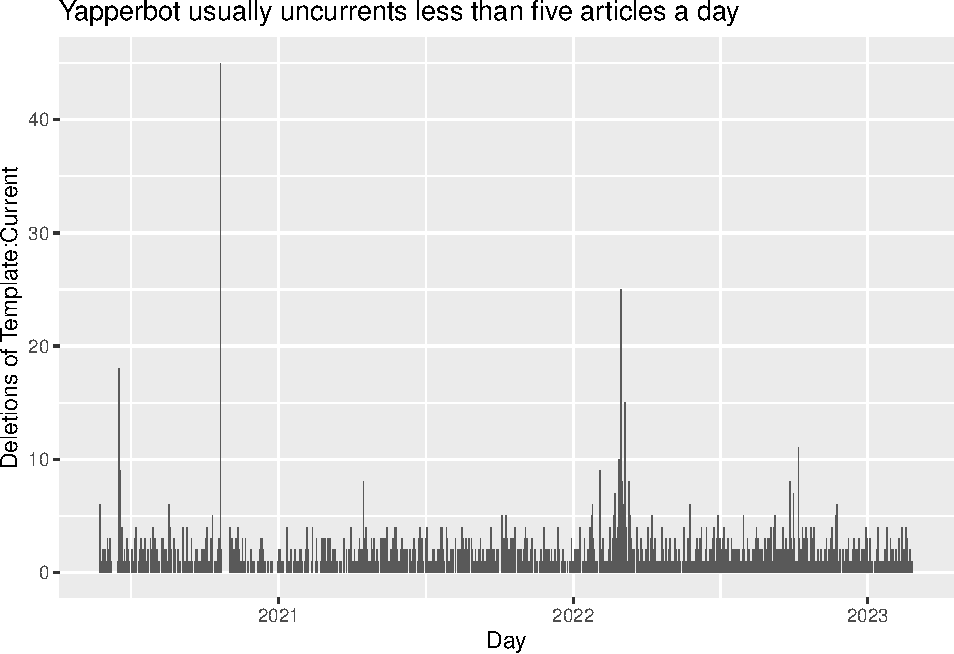
\includegraphics[width=1\linewidth]{the-bot-that-makes-history_files/figure-latex/unnamed-chunk-3-1}

What was happening on that day it uncurrented 45 pages?

\begin{verbatim}
## # A tibble: 45 x 3
##      pageid title                                            timestamp          
##       <dbl> <chr>                                            <dttm>             
##  1 63362621 COVID-19 pandemic in Ethiopia                    2020-10-21 23:00:28
##  2 63431783 COVID-19 pandemic in Northern Ireland            2020-10-21 22:00:48
##  3 63181042 COVID-19 pandemic in Europe                      2020-10-21 22:00:41
##  4 63178596 COVID-19 pandemic in Hong Kong                   2020-10-21 22:00:38
##  5 63313047 COVID-19 pandemic in Moldova                     2020-10-21 21:00:43
##  6 63239190 COVID-19 pandemic in Sweden                      2020-10-21 21:00:37
##  7 64307024 Timeline of the COVID-19 pandemic in October 20~ 2020-10-21 20:00:49
##  8 63395521 COVID-19 pandemic in Sarawak                     2020-10-21 20:00:45
##  9 63391509 COVID-19 pandemic in Quebec                      2020-10-21 20:00:39
## 10 63389195 COVID-19 pandemic in Sabah                       2020-10-21 20:00:36
## # i 35 more rows
\end{verbatim}

How often does Yapperbot have to remove the template more than once?

\begin{verbatim}
## # A tibble: 7 x 2
##   count num_pages
##   <int>     <int>
## 1     1      1236
## 2     2       133
## 3     3        23
## 4     4         9
## 5     5         4
## 6     6         2
## 7     9         1
\end{verbatim}

Which page had to be uncurrented nine times?

\begin{verbatim}
## `summarise()` has grouped output by 'pageid'. You can override using the
## `.groups` argument.
\end{verbatim}

\begin{verbatim}
## # A tibble: 7 x 3
## # Groups:   pageid [7]
##     pageid title                                            count
##      <dbl> <chr>                                            <int>
## 1 70168267 Siege of Mariupol                                    9
## 2 65760352 Tigray War                                           6
## 3 70161957 Siege of Chernihiv                                   6
## 4 64399515 2020–2021 Belarusian protests                        5
## 5 70157964 Timeline of the 2022 Russian invasion of Ukraine     5
## 6 70160923 Battle of Kharkiv (2022)                             5
## 7 70809573 2022–2023 monkeypox outbreak                         5
\end{verbatim}

\hypertarget{wikipedia-time-2-encyclopaedia-time}{%
\section{Wikipedia time (2): encyclopaedia
time}\label{wikipedia-time-2-encyclopaedia-time}}

\emph{Compared to other temporal regimes}

\bibliographystyle{sageh}
\bibliography{wikihistories.bib}


\end{document}
